\documentclass{beamer}

\usepackage{pdfpc-movie}
\usepackage{svg}

\usetheme{Boadilla}

% Title
\title{LUG General Body Meet}
\author{Ethan Wong \and Harshit Modi}
\date{\today}
\institute{Linux Users Group @ UIC}

\begin{document}
\begin{frame}
	\titlepage
\end{frame}

\begin{frame}{Table of Contents}
	\tableofcontents[pausesections]
\end{frame}

\section{What is LUG?}
\begin{frame}{Linux User Group @ UIC}
	\begin{columns}
		\begin{column}{0.5\textwidth}
			\begin{figure}
				\centering
				\includegraphics[width=0.75\textwidth]{lug-logo.png}
			\end{figure}
		\end{column}
		\begin{column}{0.5\textwidth}
			LUG stands for \underline{Linux User's Group}.
			\pause We are a pre-professional organization who's mission is to
			provide a community space for like-minded individuals with interests
			in:
			\begin{itemize}
				\item Linux
				\item Free and Open Source Software
				\item Hardware Hacking
				\item Privacy and Security
				\item \textit{among others...}
			\end{itemize}
		\end{column}
	\end{columns}
\end{frame}

\begin{frame}{Fun Facts}
	\begin{itemize}
		\item We are one of the oldest student organizations in the University,
		      next to \textbf{ACM}, our sister organization.
		      \pause
		      \begin{figure}
			      \centering
			      \includegraphics[width=0.60\textwidth]{site_history.png}
			      \caption{Our website has been active since 2006!}
		      \end{figure}
		      \pause
		\item We share an office with ACM in \underline{SELE 2264}
		      where \textit{anyone} can come in and talk technology!
		      \pause
		\item We maintain one of the largest CS org Discord servers,
			nearing \textbf{600} members :D
	\end{itemize}
\end{frame}

\subsection{Meet the Officers}
\begin{frame}{Meet the Officers}
	{\Huge President}
	\begin{columns}
		\begin{column}{0.5\textwidth}
			\begin{itemize}
				\item {\Large Ethan Wong}
				\item Contact:
				      \href{mailto:ewong25@uic.edu}{\texttt{ewong25@uic.edu}}
				\item Maintaining LUG since 2024
				      \begin{itemize}
					      \item Distro: Arch
					      \item Owns \textit{too many} Thinkpads
					      \item Loves homelabbing and enterprise rack-servers
					      \item Interested in VR hardware
				      \end{itemize}
			\end{itemize}
		\end{column}
		\begin{column}{0.5\textwidth}
			\begin{figure}
				\centering
				\includegraphics[width=0.9\textwidth,angle=270]{neko-homelab.jpg}
				\caption{My Homelab}
			\end{figure}
		\end{column}
	\end{columns}
\end{frame}

\begin{frame}{Meet the Officers}
	{\Huge Vice President}
	\begin{columns}
		\begin{column}{0.5\textwidth}
			\begin{itemize}
				\item {\Large Jacob Cohen}
				\item Contact:
				      \href{mailto:jcohen30@uic.edu}{\texttt{jcohen30@uic.edu}}
				\item Maintaining LUG since 2024
				      \begin{itemize}
					      \item Distro: Debian 12 on Home PC
					      \item PhD Student under Professor Eriksson
					      \item Runs ACM's SIG Systems
				      \end{itemize}
			\end{itemize}
		\end{column}
		\begin{column}{0.5\textwidth}
			\begin{figure}
				\centering
				\pdfpcmovie[width=\textwidth,height=\textwidth,autostart,loop]{}{linux-kernel.mp4}
			\end{figure}
		\end{column}
	\end{columns}
\end{frame}

\begin{frame}{Meet the Officers}
	{\Huge Officer}
	\begin{columns}
		\begin{column}{0.5\textwidth}
			\begin{itemize}
				\item {\Large Harshit "Harsh" Modi} — LUG guy since 2025.
				\item {\scriptsize \href{mailto:hmodi5@uic.edu}{hmodi5@uic.edu}} — Email me, I might reply.
				\item {\small Fedora user} — Arch is pain, Ubuntu is boring.
				\item {\small \url{https://justharsh.xyz/}} — It exists.
				\item Runs on caffeine and regret.
				\item No homelab \includegraphics[width=1em]{cry_emoji.png} — wallet said no.
			\end{itemize}
		\end{column}
		\begin{column}{0.5\textwidth}
			\centering
			\includegraphics[width=0.8\textwidth]{drunk_tux.jpg}
		\end{column}
	\end{columns}
\end{frame}

\begin{frame}{Meet the Officers}
	{\Huge Officer}
	\begin{columns}
		\begin{column}{0.5\textwidth}
			\begin{itemize}
				\item {\Large Michael Hanif Khan}
				\item Maintaining LUG since 2025!
				\item Contact
				      \begin{itemize}
					      \item Email: \href{mailto:mkhan398@uic.edu}{mkhan398@uic.edu}
					      \item Discord: @milknolactose
					      \item Website: \href{https://xmasscan.github.io/index.html}{xmasscan.github.io}
				      \end{itemize}
				\item Jumped from WSL to Arch
				\item Interested in learning about Computer Security and setting up servers!
				\item Reluctant Weezer fan, respectable Jeff Rosenstock fan
			\end{itemize}
		\end{column}
		\begin{column}{0.5\textwidth}
			\centering
			\includegraphics[width=0.8\textwidth]{snake.png}
		\end{column}
	\end{columns}
\end{frame}

\begin{frame}{Contact Us}
	\Huge Email us!
	\href{mailto:lug-officers@uic.edu}{\texttt{lug-officers@uic.edu}}
\end{frame}

\section{What's Linux?}
\begin{frame}{Table of Contents}
	\tableofcontents[currentsection]
\end{frame}

\begin{frame}{What's Linux?}
	\begin{columns}
		\begin{column}{0.5\textwidth}
			\textbf{Linux} is a free and open-source operating
			system kernel. Linux is part of a family of operating
			systems that bundle various pieces of software to form
			a complete OS, called \underline{Linux distros}.
		\end{column}
		\begin{column}{0.5\textwidth}
			\begin{figure}
				\centering
				\includesvg[width=0.9\textwidth]{tux.svg}
				\caption{Tux, the Linux mascot}
			\end{figure}
		\end{column}
	\end{columns}
\end{frame}

\subsection{Why Linux?}
\begin{frame}{Why Linux?}
	\begin{itemize}
		\item It's truly free!
		      \pause
		      \begin{itemize}
			      \item Anyone can view, modify, and redistribute
			            the the kernel and its underlying
			            source code.
			            \pause
			      \item It's actually libre/available for no
			            charge.\footnote{most of the time}
			            \pause
		      \end{itemize}
		\item Linux powers millions of devices like Android
		      smartphones, Chromebooks, and even the \textbf{top 500}
		      supercomputers in the world!
		      \pause
		\item Unix-like systems like Linux are widespread in academia.
		      Learning its usage is beneficial to your research and
		      coursework!
		      \pause
		\item Linux systems are tailored to software development,
		      programming and installing dependencies is far easier
		      on Linux than other operating systems.
		      \pause
		\item It's \underline{not} Windows.
		      \pause
		      \begin{itemize}
			      \item Or macOS either...
		      \end{itemize}
		      \pause
	\end{itemize}
	Curious? Check out our Linux Week event coming soon!\footnote{will be
		announced later in the presentation}
\end{frame}

\section{What We've Been Up To}
\begin{frame}{Table of Contents}
	\tableofcontents[currentsection]
\end{frame}

\begin{frame}{Past Presentations}
	In the past, we've ran presentations/workshops on various topics to
	spread knowledge of how to better use a Linux system. Some of these
	include:
	\pause
	\begin{itemize}
		\item Vim, the ubiquitous text editor
		      \pause
		\item SystemD, the system and service manager
		      \pause
		\item Makefiles
		      \pause
		\item GDB
		      \pause
		\item \textit{and more...}
		      \pause
	\end{itemize}
	You may have even encountered these in your coursework!
\end{frame}

\begin{frame}{Website}
	\begin{columns}
		\begin{column}{0.4\textwidth}
			\begin{figure}
				\centering
				\includegraphics[width=\textwidth]{website.png}
				\caption{LUG Website}
			\end{figure}
		\end{column}
		\begin{column}{0.6\textwidth}
			We've been building a \textit{community-contributed}
			knowledge-base for Linux users at UIC who...
			\pause
			\begin{itemize}
				\item \underline{daily-drive} Linux
				      \pause
				\item use Linux in a class (i.e.
				      \texttt{systems\{1..4\}.cs.uic.edu})
				      \pause
				\item need information about Linux, GNU, Free
				      Software, etc. or are otherwise trying
				      to learn
				      \pause
			\end{itemize}
			Our new website has been in active development since
			\textbf{2022}. Students are also free to contribute,
			our website is open source under the MIT license. Check
			it out! \url{https://lug.cs.uic.edu}
		\end{column}
	\end{columns}
\end{frame}

\begin{frame}{Projects}
	We've been working on fun things within the ACM/LUG room, mostly
	hobbyist projects that \textit{anyone} can get involved with!
	\pause
	\begin{figure}
		\centering
		\pdfpcmovie[width=0.7\textwidth,height=0.39375\textwidth]{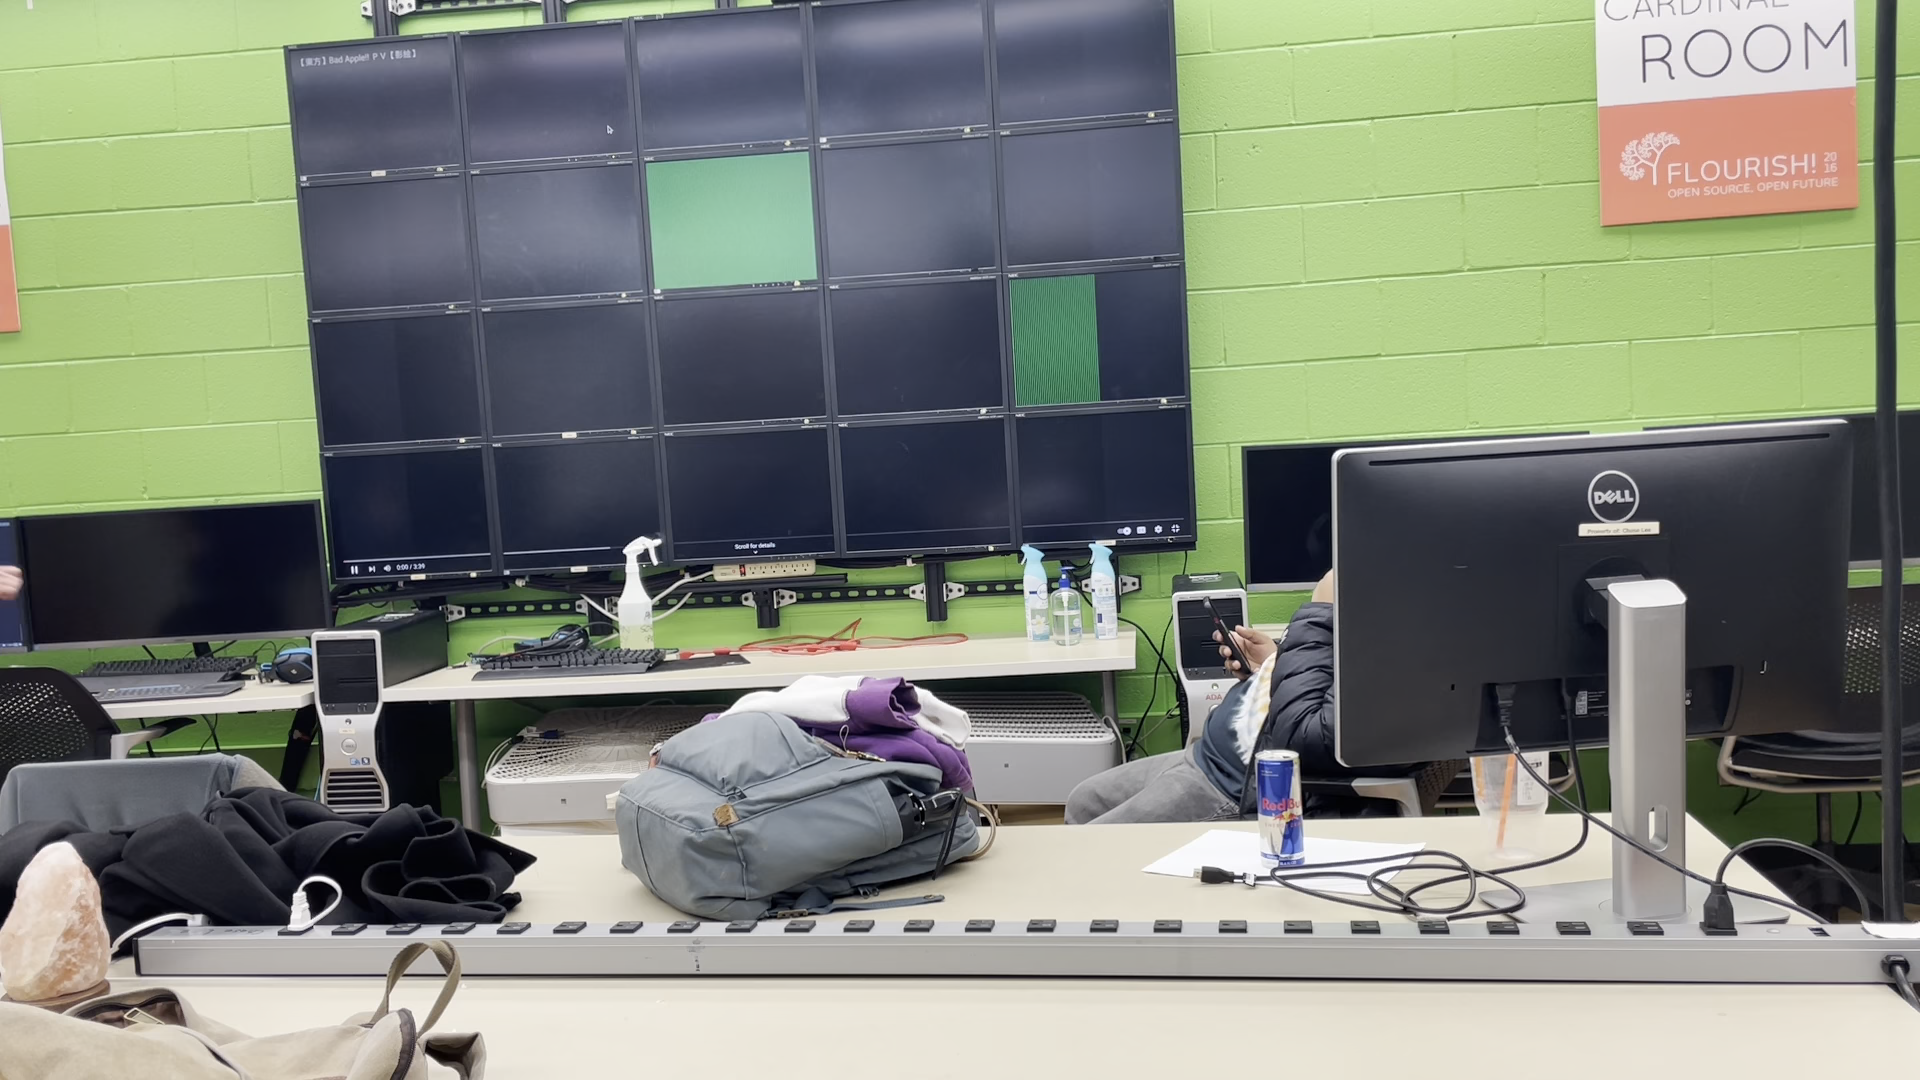
\includegraphics[width=0.7\textwidth]{bad-apple.png}}{bad-apple.mp4}
		\caption{Bad Apple on the Monitor Wall
			(\url{https://www.youtube.com/watch?v=IMMLflKIPig})}
	\end{figure}
\end{frame}

\begin{frame}{Projects}
	Apart from that, our GitHub has many of our open-source works,
	including:
	\pause
	\begin{itemize}
		\item Cerberus, an LDAP user management app
		      \pause
		\item \texttt{eventfetch}, automated event flyers
		      \pause
		\item \texttt{doorkeeper-driver}, an evdev driver for keycard
		      readers
		      \pause
		\item \texttt{doorbot}, a Discord bot to keep access in the
		      ACM/LUG office
		      \pause
	\end{itemize}
	Among many other incomplete works lost in the weeds due to time. Check
	it out here: \url{https://github.com/lugatuic}.
\end{frame}

\begin{frame}{Server Rack}
	\begin{columns}
		\begin{column}{0.4\textwidth}
			\begin{figure}
				\centering
				\includegraphics[width=0.9\textwidth]{server.jpg}
				\caption{ACM/LUG Server Room}
			\end{figure}
		\end{column}
		\begin{column}{0.6\textwidth}
			We share a server rack with \textbf{ACM}. \pause We own
			our own server on the rack: \texttt{miku}.
			\texttt{miku} is a Dell Poweredge R610 running Proxmox,
			a KVM-based hypervisor which manages virtual machines.
			This server has an overkill amount of hardware.
		\end{column}
	\end{columns}
\end{frame}

\begin{frame}{Try Linux Without Reimaging!}
	\textbf{Not ready to install Linux on your computer yet? No worries!}
	\pause
	\begin{itemize}
		\item You can use \textbf{Windows Subsystem for Linux (WSL)} to run a full Linux environment inside Windows.
			\begin{itemize}
				\item Great for developers who want access to Linux tools without dual-booting.
				\item Supports package management, shell scripting, and much more!
			\end{itemize}
		\pause
		\item Alternatively, \textbf{LUG can provide you with a virtual machine (VM)} to safely explore Linux without touching your main system.
			\begin{itemize}
				\item A pre-configured Linux VM for you to experiment with.
				\item Perfect for beginners who want hands-on experience.
			\end{itemize}
		\pause
	\end{itemize}
	Reach out to us on discord if you're interested!
\end{frame}


\section{Future Plans}
\begin{frame}{Table of Contents}
	\tableofcontents[currentsection]
\end{frame}

\begin{frame}{Tentative Semester Presentations}
	We're proud to offer these topics as workshops this semester.
	\pause
	\begin{itemize}
		\item Thinkpads and Linux by Ethan
		\item Build and deploy website with Hugo and Github Pages by Jacob
		\item Filesystem by Harshit
        \textit{and many more}
	\end{itemize}
	\pause
	\textit{If you want a specific topic covered or want to present your
		own presentation, let us know!
		\href{mailto:lug-officers@uic.edu}{\texttt{lug-officers@uic.edu}}}
\end{frame}

\begin{frame}{The Endless To-Do List}
	We have some projects we'd like to get done, and we need help! If any
	of these interest you, feel free to reach out to us.\footnote{
		\href{mailto:lug-officers@uic.edu}{\texttt{lug-officers@uic.edu}}}
	\pause

	\begin{itemize}
		\item Re-image \texttt{chopin}, a legacy server on the ACM/LUG
		      server rack.
		\item Spin-up a Matrix homeserver and \underline{bridge} it
		      with the Discord.
		\item Migrate our website off Github Pages and onto our own
		      server.
		\item Add features to our website like a sidebar and search.
	\end{itemize}
\end{frame}

\section{How To Get Involved}
\begin{frame}{Table of Contents}
	\tableofcontents[currentsection]
\end{frame}

\begin{frame}{Join our Discord!}
	\begin{figure}
		\centering
		\includesvg[width=0.5\textwidth]{lug-discord.svg}
		\caption{\url{https://discord.gg/NgxTR7PX5e}}
	\end{figure}
\end{frame}

\begin{frame}{I Hate Discord \>:(}
	\textbf{We also have a \textit{newsletter listserv}!}

	Email \texttt{SUBSCRIBE LUG} to
	\href{mailto:listserv@uic.edu}{\texttt{listserv@uic.edu}} for timely
	email notifications.

	Also, you should join CampusGroups to be ``officially'' part of the club.

	\url{https://uic.campusgroups.com/linuxuser/club\_signup}
\end{frame}

\begin{frame}{We're Hiring!}
	As mentioned previously, \underline{we want people to help contribute
		to LUG!} \pause If you want to help with projects or have a
	presentation you want to present, email
	\href{mailto:lug-officers@uic.edu}{\texttt{lug-officers@uic.edu}} or DM
	us on Discord :D
\end{frame}

\begin{frame}{Closing Remarks}
	\begin{center}
		{\Huge Thank you!}

		\textit{We'll stick around to chat afterwards...}
	\end{center}
\end{frame}

\begin{frame}{Closing Remarks}
	\begin{columns}
		\begin{column}{0.5\textwidth}
			\textbf{Officers}
			\begin{figure}
				\centering
				\includegraphics[width=0.60\textwidth]{officers.png}
			\end{figure}
		\end{column}
		\begin{column}{0.5\textwidth}
			The information in this presentation will be made
			available\footnotemark on our website!\\
			\url{https://lug.cs.uic.edu}

			\bigskip
			Join our Discord!

			\begin{figure}
				\centering
				\includesvg[width=0.5\textwidth]{lug-discord.svg}
				\caption{\url{https://discord.gg/NgxTR7PX5e}}
			\end{figure}
		\end{column}
	\end{columns}

	\footnotetext{sooner or later}
\end{frame}

\end{document}

% vim: set tw=80 ts=4 sw
